% 原书第3--8页至题型一结束；PDF第11--16页。人工对照原页转写。
\chapter{矩阵与线性变换}
高等代数内容包括：线性代数和多项式。本章重点关注矩阵与线性变换。
由于线性变换可用矩阵表示，本质上讲研究线性变换也就是研究矩阵。
因此我们讨论的主要内容包括矩阵的运算、线性变换的基本性质，以及矩阵的行列式、矩阵的特征值和特征向量、矩阵的秩、矩阵的迹等。
这些是线性代数的基础部分，特别地，矩阵与行列式是两个最基本的概念，熟练掌握它们的性质是最基本的要求。

\section{竞赛要点与难点}
\begin{enumerate}[label=（\arabic*）]
\item 矩阵的概念，矩阵的运算（加法、数乘、乘法、转置等运算）及其运算律。
\item 矩阵乘积的行列式、矩阵乘积的秩与其因子的秩的关系。
\item 矩阵的逆、伴随矩阵、矩阵可逆的条件，初等矩阵、初等变换、矩阵的等价标准形及逆矩阵的求解等。
\item 分块矩阵：分块矩阵及其运算与性质，分块初等矩阵、分块初等变换及其应用等。
\item 行列式的定义：2阶、3阶行列式的定义及对角线法则，排列与逆序数，$n$级行列式的定义等。
\item 行列式的性质。
\item 行列式的计算：根据定义计算行列式，利用行列式性质计算行列式，行列式行（列）展开、Laplace（拉普拉斯）展开定理等。
\item Cramer（克拉默）法则。
\item 矩阵的行秩、列秩、秩、矩阵的秩与其子式的关系。
\item 线性变换的定义、线性变换的运算、线性变换的矩阵。
\item 特征值与特征向量：线性变换和矩阵的特征值与特征向量、可对角化线性变换和矩阵的性质与判定、相似矩阵、相似不变量、Hamilton--Cayley（哈密顿--凯莱）定理等。
\item $\lambda$-矩阵：$\lambda$-矩阵、$\lambda$-矩阵在初等变换下的标准形、行列式因子、不变因子、初等因子，矩阵相似的条件等。
\item Jordan（若尔当）矩阵、Jordan标准形、有理标准形。
\end{enumerate}

\section{范例解析与精讲}
\subsection*{题型一\quad 矩阵的运算}
矩阵的运算中需要注意矩阵乘法不满足交换律，同时矩阵中有零因子存在，即两个非零矩阵乘积可以等于零矩阵。概括起来，以下几点需要特别注意：
\begin{enumerate}[label=（\arabic*）]
\item 一般地，二项式定理
\[
(A+B)^n=\sum_{i=0}^n\binom ni A^iB^{n-i}
\]
不一定成立。但若$A,B$可交换，即$AB=BA$，则上式成立。
\item 矩阵乘法没有消去律，即$CX=CY$（或$XC=YC$）推不出$X=Y$。但是有如下特别结论：
\begin{enumerate}[label=（\roman*）]
\item 一个矩阵$C$左可消当且仅当$C$为列满秩，即以下两条陈述等价：
\begin{enumerate}[label=（\alph*）]
\item 由$CX=CY$可推出$X=Y$。
\item $C$是列满秩，即$C$的列向量组线性无关或者$\rank(C)=C$的列数。
\end{enumerate}
\item 一个矩阵$C$右可消当且仅当$C$为行满秩，即以下两条陈述等价：
\begin{enumerate}[label=（\alph*）]
\item 由$XC=YC$可推出$X=Y$。
\item $C$是行满秩，即$C$的行向量组线性无关或者$\rank(C)=C$的行数。
\end{enumerate}
\item $A^2=E$推不出$A=E$或$A=-E$，即$A^2-E=(A+E)(A-E)=O$推不出$A+E=O$或$A-E=O$。
\end{enumerate}
\end{enumerate}

\ex{1.2.1}设$A,B$均是$n$阶方阵且满足$A^2=A$，$B^2=B$，$(A+B)^2=A+B$，求$AB$。
\sol 由$(A+B)^2=A+B$得到
\[A^2+AB+BA+B^2=A+B.\]
又$A^2=A$，$B^2=B$，所以
\[AB=-BA,\]
从而
\[A\cdot AB=-A\cdot BA,\]
即
\[AB=-ABA;\]
\[AB\cdot A=-BA\cdot A,\]
即
\[ABA=-BA\quad\text{或}\quad BA=-ABA,\]
因此
\[AB=BA.\]
由此得到$2AB=O$，故有$AB=O$。

\ex{1.2.3}设
\[
A=\begin{pmatrix}
a_1b_1&a_1b_2&\cdots&a_1b_n\\
a_2b_1&a_2b_2&\cdots&a_2b_n\\
\vdots&\vdots&&\vdots\\
a_nb_1&a_nb_2&\cdots&a_nb_n
\end{pmatrix},
\]
$k$为正整数，求$A^k$。
\sol $A$可分解为
\[
A=\begin{pmatrix}a_1\\a_2\\\vdots\\a_n\end{pmatrix}
\begin{pmatrix}b_1&b_2&\cdots&b_n\end{pmatrix}
=\alpha\beta^{\mathrm T},
\]
其中
\[
\alpha=\begin{pmatrix}a_1\\a_2\\\vdots\\a_n\end{pmatrix},\qquad
\beta=\begin{pmatrix}b_1\\b_2\\\vdots\\b_n\end{pmatrix},
\]
所以
\begin{align*}
A^k&=\underbrace{(\alpha\beta^{\mathrm T})(\alpha\beta^{\mathrm T})\cdots(\alpha\beta^{\mathrm T})}_{k\text{个}}\\
&=\alpha\underbrace{(\beta^{\mathrm T}\alpha)(\beta^{\mathrm T}\alpha)\cdots(\beta^{\mathrm T}\alpha)}_{k-1\text{个}}\beta^{\mathrm T}\\
&=\alpha(\beta^{\mathrm T}\alpha)^{k-1}\beta^{\mathrm T},
\end{align*}
而
\[\beta^{\mathrm T}\alpha=a_1b_1+a_2b_2+\cdots+a_nb_n,\]
故有
\begin{align*}
A^k&=(a_1b_1+a_2b_2+\cdots+a_nb_n)^{k-1}A\\
&=(a_1b_1+a_2b_2+\cdots+a_nb_n)^{k-1}
\begin{pmatrix}
a_1b_1&a_1b_2&\cdots&a_1b_n\\
a_2b_1&a_2b_2&\cdots&a_2b_n\\
\vdots&\vdots&&\vdots\\
a_nb_1&a_nb_2&\cdots&a_nb_n
\end{pmatrix}.
\end{align*}

\ex{1.2.5}设
\[
A=\begin{pmatrix}
2&0&0&0&0&0\\
3&2&0&0&0&0\\
0&3&2&0&0&0\\
0&0&0&1&2&0\\
0&0&0&0&1&2\\
0&0&0&0&0&1
\end{pmatrix},
\]
求$A^{100}$。
\sol 设
\[
A_1=\begin{pmatrix}2&0&0\\3&2&0\\0&3&2\end{pmatrix},\qquad
A_2=\begin{pmatrix}1&2&0\\0&1&2\\0&0&1\end{pmatrix}.
\]
则$A$可写为如下分块形式：
\[A=\begin{pmatrix}A_1&\\&A_2\end{pmatrix},\]
于是
\[A^{100}=\begin{pmatrix}A_1^{100}&\\&A_2^{100}\end{pmatrix}.\]
将$A_1,A_2$分解为
\[
A_1=2E+3S,\qquad\text{其中}\quad
S=\begin{pmatrix}0&0&0\\1&0&0\\0&1&0\end{pmatrix};
\]
\[
A_2=E+2H,\qquad\text{其中}\quad
H=\begin{pmatrix}0&1&0\\0&0&1\\0&0&0\end{pmatrix}.
\]
注意到$S$与$E$、$H$与$E$均可交换且
\[
S^2=\begin{pmatrix}0&0&0\\0&0&0\\1&0&0\end{pmatrix},\qquad
S^i=O\quad(i\ge3),
\]
\[
H^2=\begin{pmatrix}0&0&1\\0&0&0\\0&0&0\end{pmatrix},\qquad
H^i=O\quad(i\ge3).
\]
由二项式定理
\begin{align*}
A_1^{100}
&=(2E+3S)^{100}=\sum_{i=0}^{100}\binom{100}{i}(2E)^{100-i}(3S)^i\\
&=\binom{100}{0}(2E)^{100}
 +\binom{100}{1}(2E)^{99}\cdot3S
 +\binom{100}{2}(2E)^{98}(3S)^2\\
&=2^{100}E+300S\cdot2^{99}E
 +\frac{100\times99}{2}\cdot9S^2\cdot2^{98}E\\
&=2^{100}E+300\cdot2^{99}\cdot S+50\cdot99\cdot9\cdot2^{98}\cdot S^2\\
&=\begin{pmatrix}
2^{100}&0&0\\
3\cdot5^2\cdot2^{101}&2^{100}&0\\
11\cdot5^2\cdot3^4\cdot2^{99}&3\cdot5^2\cdot2^{101}&2^{100}
\end{pmatrix},
\end{align*}
\begin{align*}
A_2^{100}
&=(E+2H)^{100}
 =E^{100}+100\cdot E^{99}\cdot(2H)
 +\frac{100\times99}{2}\cdot E^{98}\cdot(2H)^2\\
&=E+200H+19800H^2\\
&=\begin{pmatrix}1&200&19800\\0&1&200\\0&0&1\end{pmatrix}.
\end{align*}
因此
\[
\setlength{\arraycolsep}{3pt}
A^{100}=\begin{pmatrix}
2^{100}&0&0&0&0&0\\
3\cdot5^2\cdot2^{101}&2^{100}&0&0&0&0\\
11\cdot5^2\cdot3^4\cdot2^{99}&3\cdot5^2\cdot2^{101}&2^{100}&0&0&0\\
0&0&0&1&200&19800\\
0&0&0&0&1&200\\
0&0&0&0&0&1
\end{pmatrix}.
\]

\par\medskip\noindent\textbf{总结}\quad 计算方阵的方幂一般有三种方法：
\begin{enumerate}[label=（\arabic*）]
\item 基于相似变换的计算法。更常见的情形是利用相似标准形（比如Jordan标准形）来进行计算。
\item 利用递推公式法或者说数学归纳法，如例1.2.3。
\item 基于方阵分解，然后利用二项式定理来进行计算，如例1.2.5。
\end{enumerate}

% SOURCE_PDF_PAGE 14

\par\medskip\noindent \raisebox{-4.33pt}{
\includegraphics[width=106.45pt]{images/p014-b000.png}}

\typeout{OCRFORM p014-b001}\eq{\boldsymbol{A}=\left( \begin{array} {c c c c c c} {2} & {0} & {0} & {0} & {0} & {0} \\ {3} & {2} & {0} & {0} & {0} & {0} \\ {0} & {3} & {2} & {0} & {0} & {0} \\ {0} & {0} & {0} & {1} & {2} & {0} \\ {0} & {0} & {0} & {0} & {1} & {2} \\ {0} & {0} & {0} & {0} & {0} & {1} \\ \end{array} \right) ,}


% SOURCE_PDF_PAGE 15
求\typeout{OCRFORM p015-b001}$\boldsymbol{A}^{1 0 0}$。
\sol 设
\typeout{OCRFORM p015-b004}\eq{\boldsymbol{A}_{1}=\left( \begin{array} {c c c} {2} & {0} & {0} \\ {3} & {2} & {0} \\ {0} & {3} & {2} \\ \end{array} \right) , \quad\boldsymbol{A}_{2}=\left( \begin{array} {c c c} {1} & {2} & {0} \\ {0} & {1} & {2} \\ {0} & {0} & {1} \\ \end{array} \right) .}

则\typeout{OCRFORM p015-b006}$\boldsymbol{A}$可写为如下分块形式:

\typeout{OCRFORM p015-b008}\eq{{\boldsymbol A}=\left( \begin{array} {c c} {{\boldsymbol A}_{1}} & {} \\ {} & {{\boldsymbol A}_{2}} \\ \end{array} \right) \! ,}

于是

\typeout{OCRFORM p015-b010}\eq{{\boldsymbol A}^{1 0 0}=\left( \begin{array} {c c} {{\boldsymbol A}_{1}^{1 0 0}} & {{}} \\ {{}} & {{\boldsymbol A}_{2}^{1 0 0}} \\ \end{array} \right) \! .}

将\typeout{OCRFORM p015-b012}$\boldsymbol{A}_{1} , \boldsymbol{A}_{2}$分解为
\typeout{OCRFORM p015-b014}$\boldsymbol{A}_{1}=2 \boldsymbol{E}+3 \boldsymbol{S}$，其中\typeout{OCRFORM p015-b016}$\boldsymbol{S}=\left( \begin{array} {c c c} {0} & {0} & {0} \\ {1} & {0} & {0} \\ {0} & {1} & {0} \\ \end{array} \right) \! ;$
\typeout{OCRFORM p015-b017}$\boldsymbol{A}_{2}=\boldsymbol{E}+2 \boldsymbol{H}$，其中\typeout{OCRFORM p015-b019}$\boldsymbol{H}=\left( \begin{array} {c c c} {0} & {1} & {0} \\ {0} & {0} & {1} \\ {0} & {0} & {0} \\ \end{array} \right) \! .$
注意到\raisebox{-2.92pt}{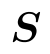
\includegraphics[width=13.98pt]{images/p015-b021.png}}与\raisebox{-3.12pt}{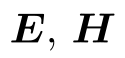
\includegraphics[width=34.98pt]{images/p015-b023.png}}与\raisebox{-2.87pt}{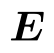
\includegraphics[width=14.99pt]{images/p015-b025.png}}均可交换且
\raisebox{-5.00pt}{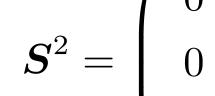
\includegraphics[width=60.42pt]{images/p015-b027.png}}
\typeout{OCRFORM p015-b028}\eq{\left( \begin{array} {c c} {0} & {0} \\ {0} & {0} \\ {0} & {0} \\ \end{array} \right) , \quad\boldsymbol{S}^{i}=\boldsymbol{O} \ ( i \geqslant3 ) , \quad\boldsymbol{H}^{2}=\left( \begin{array} {c c c} {0} & {0} & {1} \\ {0} & {0} & {0} \\ {0} & {0} & {0} \\ \end{array} \right) , \quad\boldsymbol{H}^{i}=\boldsymbol{O} \ ( i \geqslant3 ) .}

0
1
由二项式定理

\typeout{OCRFORM p015-b032}\eq{\begin{aligned} {\boldsymbol{A}_{1}^{1 0 0}} & {{}=( 2 \boldsymbol{E}+3 \boldsymbol{S} )^{1 0 0}=\sum_{i=0}^{1 0 0} \binom{1 0 0} {i} ( 2 \boldsymbol{E} )^{1 0 0-i} ( 3 \boldsymbol{S} )^{i}} \\ {} & {{}=\binom{1 0 0} {0} ( 2 \boldsymbol{E} )^{1 0 0}+\binom{1 0 0} {1} ( 2 \boldsymbol{E} )^{9 9} \cdot3 \boldsymbol{S}+\binom{1 0 0} {2} ( 2 \boldsymbol{E} )^{9 8} ( 3 \boldsymbol{S} )^{2}} \\ {} & {{}=2^{1 0 0} \boldsymbol{E}+3 0 0 \boldsymbol{S} \cdot2^{9 9} \boldsymbol{E}+\frac{1 0 0 \times9 9} {2} \cdot9 \boldsymbol{S}^{2} \cdot2^{9 8} \boldsymbol{E}} \\ {} & {{}=2^{1 0 0} \boldsymbol{E}+3 0 0 \cdot2^{9 9} \cdot\boldsymbol{S}+5 0 \cdot9 9 \cdot9 \cdot2^{9 8} \cdot\boldsymbol{S}^{2}} \\ \end{aligned}}


% SOURCE_PDF_PAGE 16

\typeout{OCRFORM p016-b000}\eq{= \left( \begin{array} {c c c} {2^{1 0 0}} & {0} & {0} \\ {3 \cdot5^{2} \cdot2^{1 0 1}} & {2^{1 0 0}} & {0} \\ {1 1 \cdot5^{2} \cdot3^{4} \cdot2^{9 9}} & {3 \cdot5^{2} \cdot2^{1 0 1}} & {2^{1 0 0}} \\ \end{array} \right) ,}


\typeout{OCRFORM p016-b001}\eq{\begin{aligned} {\boldsymbol{A}_{2}^{1 0 0}=( \boldsymbol{E}+2 \boldsymbol{H} )^{1 0 0}} & {{}=\boldsymbol{E}^{1 0 0}+1 0 0 \cdot\boldsymbol{E}^{9 9} \cdot( 2 \boldsymbol{H} )+\frac{1 0 0 \times9 9} {2} \cdot\boldsymbol{E}^{9 8} \cdot( 2 \boldsymbol{H} )^{2}} \\ {} & {{}=\boldsymbol{E}+2 0 0 \boldsymbol{H}+1 9 8 0 0 \boldsymbol{H}^{2}} \\ {} & {{}=\left( \begin{array} {c c c} {1} & {2 0 0} & {1 9 8 0 0} \\ {0} & {1} & {2 0 0} \\ {0} & {0} & {1} \\ \end{array} \right) .} \\ \end{aligned}}

因此

\typeout{OCRFORM p016-b003}\eq{\boldsymbol{A}^{1 0 0}=\left( \begin{array} {c c c c c c} {2^{1 0 0}} & {0} & {0} & {0} & {0} & {0} \\ {3 \cdot5^{2} \cdot2^{1 0 1}} & {2^{1 0 0}} & {0} & {0} & {0} & {0} \\ {1 1 \cdot5^{2} \cdot3^{4} \cdot2^{0 9}} & {3 \cdot5^{2} \cdot2^{1 0 1}} & {2^{1 0 0}} & {0} & {0} & {0} \\ {0} & {0} & {0} & {1} & {2 0 0} & {1 9 8 0 0} \\ {0} & {0} & {0} & {0} & {1} & {2 0 0} \\ {0} & {0} & {0} & {0} & {0} & {1} \\ \end{array} \right) .}

总结 计算方阵的方幂一般有三种方法:
\par\begin{center}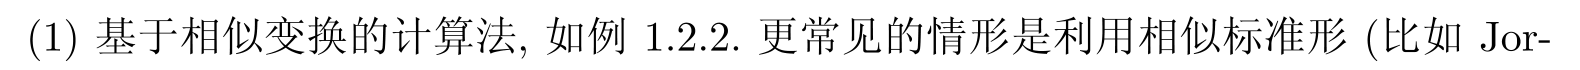
\includegraphics[width=446.01pt]{images/p016-b005.png}\end{center}
dan 标准形)来进行计算

\par\noindent (2) 利用递推公式法或者说数学归纳法，如例1. 2.3 和例1. 2 .4.

\par\noindent (3) 基于方阵分解.然后利用二项式定理来进行计算，如例1. 2 .5.
\subsection*{题型二矩阵可逆的判定及计算}
\sol 此题型常用到如下熟知的结果.
命题设\typeout{OCRFORM p016-b012}$\boldsymbol{A}$为\raisebox{-2.87pt}{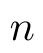
\includegraphics[width=11.95pt]{images/p016-b014.png}}阶矩阵则有
\typeout{OCRFORM p016-b016}$\boldsymbol{A}$可逆\typeout{OCRFORM p016-b018}$\Leftrightarrow\exists B$使得\typeout{OCRFORM p016-b020}$\boldsymbol{B A}=\boldsymbol{E}$
\typeout{OCRFORM p016-b021}$\Leftrightarrow\exists C$使得\typeout{OCRFORM p016-b023}$\boldsymbol{A C}=\boldsymbol{E}$
\raisebox{-3.45pt}{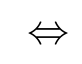
\includegraphics[width=22.87pt]{images/p016-b024.png}}\typeout{OCRFORM p016-b025}$\operatorname{r a n k} ( \boldsymbol{A} )=n$
\raisebox{-3.45pt}{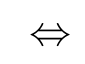
\includegraphics[width=23.57pt]{images/p016-b026.png}}\raisebox{-2.91pt}{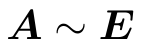
\includegraphics[width=41.05pt]{images/p016-b027.png}}
\raisebox{-3.45pt}{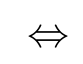
\includegraphics[width=23.19pt]{images/p016-b028.png}}\typeout{OCRFORM p016-b029}$\boldsymbol{A}$的最简行阶梯形为\raisebox{-3.02pt}{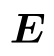
\includegraphics[width=14.89pt]{images/p016-b031.png}}
\raisebox{-3.78pt}{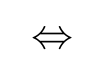
\includegraphics[width=24.31pt]{images/p016-b032.png}}\raisebox{-3.51pt}{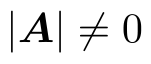
\includegraphics[width=42.26pt]{images/p016-b033.png}}
\raisebox{-3.45pt}{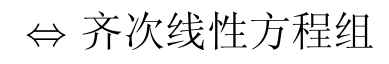
\includegraphics[width=109.52pt]{images/p016-b034.png}}\raisebox{-2.89pt}{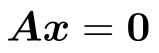
\includegraphics[width=44.68pt]{images/p016-b035.png}}只有零解
\raisebox{-3.78pt}{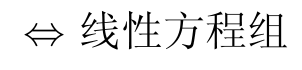
\includegraphics[width=85.02pt]{images/p016-b037.png}}\typeout{OCRFORM p016-b038}$\boldsymbol{A x}=\boldsymbol{b}$有唯一解

% SOURCE_PDF_PAGE 17
\raisebox{-3.78pt}{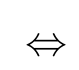
\includegraphics[width=22.07pt]{images/p017-b000.png}}\raisebox{-2.92pt}{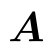
\includegraphics[width=14.95pt]{images/p017-b001.png}}的特征值均不为0
\raisebox{-3.89pt}{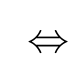
\includegraphics[width=23.01pt]{images/p017-b003.png}}\typeout{OCRFORM p017-b004}$\boldsymbol{A}$的伴随矩阵\raisebox{-3.09pt}{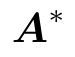
\includegraphics[width=20.81pt]{images/p017-b006.png}}可逆
\raisebox{-3.45pt}{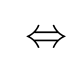
\includegraphics[width=22.40pt]{images/p017-b008.png}}\typeout{OCRFORM p017-b009}$\boldsymbol{A}$是一些初等矩阵之积.

\par\medskip\noindent 【例1. 2.6 】设\raisebox{-3.08pt}{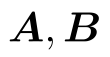
\includegraphics[width=30.77pt]{images/p017-b012.png}}均为\raisebox{-2.85pt}{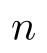
\includegraphics[width=12.87pt]{images/p017-b014.png}}阶方阵若\raisebox{-2.96pt}{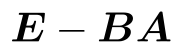
\includegraphics[width=50.85pt]{images/p017-b016.png}}可逆，证明\raisebox{-2.98pt}{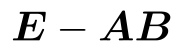
\includegraphics[width=50.45pt]{images/p017-b018.png}}可逆，并求
其逆.
\sol 考虑分块矩阵\typeout{OCRFORM p017-b022}$\left( \begin{array} {c c} {E} & {A} \\ {B} & {E} \\ \end{array} \right)$).则有'

\typeout{OCRFORM p017-b024}\eq{\left( \begin{array} {c c} {{E}} & {{-A}} \\ {{O}} & {{E}} \end{array} \right) \left( \begin{array} {c c} {{E}} & {{A}} \\ {{B}} & {{E}} \end{array} \right)=\left( \begin{array} {c c} {{E-A B}} & {{O}} \\ {{B}} & {{E}} \end{array} \right) ,}


\typeout{OCRFORM p017-b025}\eq{\left( \begin{array} {c c} {E} & {A} \\ {B} & {E} \\ \end{array} \right) \left( \begin{array} {c c} {E} & {-A} \\ {O} & {E} \\ \end{array} \right)=\left( \begin{array} {c c} {E} & {O} \\ {B} & {E-B A} \\ \end{array} \right) .}

因此

\typeout{OCRFORM p017-b027}\eq{\left| \begin{array} {c c} {E} & {A} \\ {B} & {E} \end{array} \right|=| E-A B |=| E-B A | .}

由于\raisebox{-3.08pt}{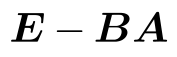
\includegraphics[width=49.62pt]{images/p017-b029.png}}可逆，即\raisebox{-3.30pt}{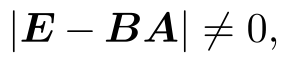
\includegraphics[width=80.27pt]{images/p017-b031.png}}，所以\raisebox{-3.26pt}{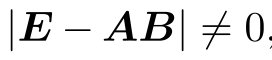
\includegraphics[width=76.72pt]{images/p017-b033.png}}\raisebox{-3.89pt}{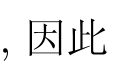
\includegraphics[width=33.56pt]{images/p017-b034.png}}\raisebox{-3.02pt}{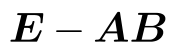
\includegraphics[width=49.29pt]{images/p017-b035.png}}可逆. 下
面进一步求(\raisebox{-3.42pt}{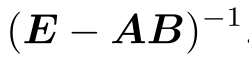
\includegraphics[width=70.11pt]{images/p017-b038.png}}. 由于

\typeout{OCRFORM p017-b040}\eq{\begin{aligned} {\boldsymbol{A} \boldsymbol{B}} & {{}=\boldsymbol{A} ( \boldsymbol{E}-\boldsymbol{B} \boldsymbol{A} ) ( \boldsymbol{E}-\boldsymbol{B} \boldsymbol{A} )^{-1} \boldsymbol{B}} \\ {} & {{}=( \boldsymbol{A}-\boldsymbol{A} \boldsymbol{B} \boldsymbol{A} ) ( \boldsymbol{E}-\boldsymbol{B} \boldsymbol{A} )^{-1} \boldsymbol{B}} \\ {} & {{}=( \boldsymbol{E}-\boldsymbol{A} \boldsymbol{B} ) \boldsymbol{A} ( \boldsymbol{E}-\boldsymbol{B} \boldsymbol{A} )^{-1} \boldsymbol{B} ,} \\ \end{aligned}}

故
\par\begin{center}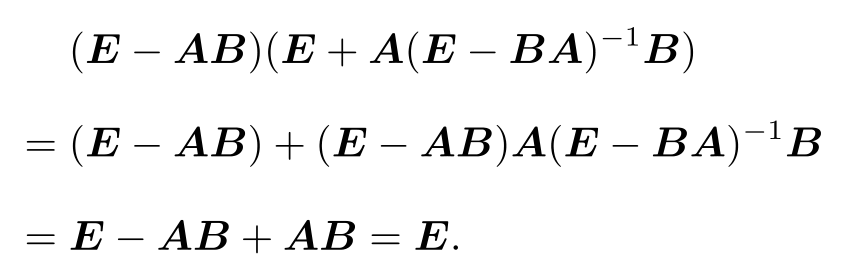
\includegraphics[width=237.75pt]{images/p017-b042.png}\end{center}
进而

\typeout{OCRFORM p017-b044}\eq{( \boldsymbol{E}-\boldsymbol{A} \boldsymbol{B} )^{-1}=\boldsymbol{E}+\boldsymbol{A} ( \boldsymbol{E}-\boldsymbol{B} \boldsymbol{A} )^{-1} \boldsymbol{B} .}


\par\medskip\noindent 【例1. 2.7 】设\typeout{OCRFORM p017-b046}$A_{1}$为\typeout{OCRFORM p017-b048}$m$阶可逆矩阵，\raisebox{-2.99pt}{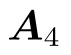
\includegraphics[width=19.90pt]{images/p017-b050.png}}为\raisebox{-2.86pt}{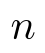
\includegraphics[width=12.26pt]{images/p017-b052.png}}阶可逆矩阵，\typeout{OCRFORM p017-b054}$A_{2}$为\typeout{OCRFORM p017-b056}$m \times n$矩阵，\typeout{OCRFORM p017-b058}$\boldsymbol{A}_{3}$
为\typeout{OCRFORM p017-b060}$n \times m$矩阵.设
